\documentclass[12pt,letterpaper]{exam}
\usepackage[lmargin=1in,rmargin=1in,tmargin=1in,bmargin=1in]{geometry}
\usepackage{../style/exams}

% -------------------
% Course & Exam Information
% -------------------
\newcommand{\course}{MAT 108: Exam 2}
\newcommand{\term}{Fall -- 2021}
\newcommand{\examdate}{11/18/2021}
\newcommand{\timelimit}{85 Minutes}

\setbool{hideans}{true} % Student: True; Instructor: False

% -------------------
% Content
% -------------------
\begin{document}

\examtitle
\instructions{Write your name on the appropriate line on the exam cover sheet. This exam contains \numpages\ pages (including this cover page) and \numquestions\ questions. Check that you have every page of the exam. Answer the questions in the spaces provided on the question sheets. Be sure to answer every part of each question and show all your work. If you run out of room for an answer, continue on the back of the page --- being sure to indicate the problem number.} 
\scores
\bottomline
\newpage

% ---------
% Questions
% ---------
\begin{questions}

% Question 1
\newpage
\question[10] Find the maximum and minimum values (if they exist) for the function $z= 5x_1 - 3x_2$ for the region shown below. 
	\[
	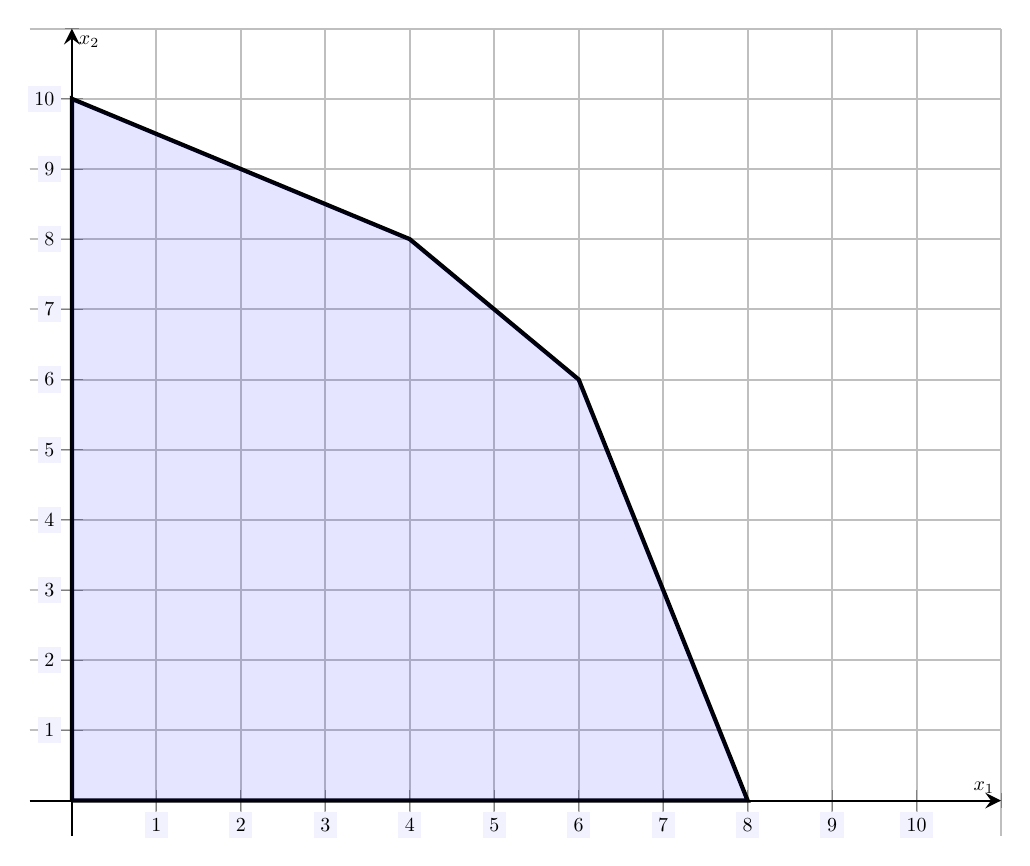
\begin{tikzpicture}[scale=1.8,every node/.style={scale=0.4}]
	\begin{axis}[
	grid=both,
	axis lines=middle,
	ticklabel style={fill=blue!5!white},
	xmin= -0.5, xmax=11,
	ymin= -0.5, ymax=11,
	xtick={-1,0,1,...,10},
	ytick={-1,0,1,...,10},
	minor tick = {-11,...,11},
	xlabel=\(x_1\),ylabel=\(x_2\),
	]
	\draw[line width=0.03cm] (0,0) -- (0,10) -- (4,8) -- (6,6) -- (8,0) -- (0,0);
	\draw[line width=0.01cm,fill= blue,opacity=0.1] (0,0) -- (0,10) -- (4,8) -- (6,6) -- (8,0) -- (0,0);
	\end{axis}
	\end{tikzpicture}
	\]





% Question 2
\newpage
\question[10] Find the tableau corresponding to the standard form of the following constrained maximization problem:
	\[
	\begin{aligned}
	\max z= 2x_1 - x_2& + 5x_3 \\
	2x_1 - x_2 + 3x_3&\leq 5 \\
	x_1 - 4x_2 - x_3&\leq 3 \\
	x_1 - x_2 - x_3&\geq 1 \\
	x_1, x_2, x_3 \geq 0
	\end{aligned}
	\]





% Question 3
\newpage
\question[10] Find the dual problem to the standard form of the following constrained minimization problem: 
	\[
	\begin{aligned}
	\min z= 4x_1 + 5x_2& + 6x_3 \\
	3x_1 - x_2 + 5x_3&\geq 6 \\
	-x_1 + 4x_2 - 2x_3&\leq 4 \\
	6x_1 + x_2 - 8x_3&\geq 7 \\
	x_1, x_2, x_3 \geq 0
	\end{aligned}
	\]





% Question 4
\newpage
\question[10] Below is the final tableau for a standard maximization problem. Find the solution to this maximization problem and find the maximum value for the function.
	\begin{table}[!ht]
	\centering
	\begin{tabular}{rrrrrrr}
	$0$ & $0.794$ & $1$ & $0.032$ & $0$ & $0.022$ & $8.868$ \\
	$0$ & $-22.608$ & $0$ & $0.038$ & $1$ & $-0.429$ & $211.935$ \\
	$1$ & $-0.195$ & $0$ & $-0.026$ & $0$ & $0.028$ & $0.699$ \\
	$0$ & $33.916$ & $0$ & $0.422$ & $0$ & $0.833$ & $212.347$
	\end{tabular}
	\end{table}





% Question 5
\newpage
\question[10] Suppose a researcher wants to create a linear model to predict a certain crop's average growth, $g$, in cm using the average number of hours of sunlight, $h$, the crops receive per day. They sample 61 different fields and collect the following data:
	\[
	\begin{aligned}
	\overline{h}&= 10 & \overline{g}&= 120 \\
	s_h^2&= 4 & s_g^2&= 64 \\
	n&= 61 & r&= 0.5
	\end{aligned}
	\] \pspace

\begin{parts}
\part Find the linear regression model to predict the growth rate using the number of hours of sunlight. \vspace{5cm}
\part Predict the average growth of crops that receive an average of 8~hours of sunlight. \vfill
\part Suppose that a crop which receives an average of 9~hours of sunlight per day grows an average of 110~cm. Find the residual for the model's prediction. Is the prediction an under or over prediction? \vfill
\part Does the average growth rate of the crops appear to be strongly correlated with the average number of hours of sunlight they receive per day? Explain. \vfill
\end{parts}





% Question 6
\newpage
\question[10] Researchers collected data on the number of running shoes sold based on the price of the shoe. Plotted below is a linear model fitted to a scatterplot of the data collected by the researchers:
	\begin{figure}[!ht]
	\centering
	\includegraphics[width=0.65\textwidth]{linreg.png}
	\end{figure} 

\begin{parts}
\part Which of the following is the most likely equation for the linear model?
	\begin{enumerate}[(i)]
	\item \usol{0.5cm}{\phantom{a}}: $\widehat{y}= 2.89x + 533$ 
	\item \usol{0.5cm}{\phantom{a}}: $\widehat{y}= -2.99x + 601.37$ 
	\item \usol{0.5cm}{\phantom{a}}: $\widehat{y}= 797.27 - 2.97x$ 
	\item \usol{0.5cm}{\phantom{a}}: $\widehat{y}= 353.70x - 67.33$ 
	\end{enumerate} \pvspace{0.2cm}
\part Which of the following is the most likely $r$ value for this model?
	\begin{enumerate}[(i)]
	\item \usol{0.5cm}{\phantom{a}}: $r= -0.9803$ 
	\item \usol{0.5cm}{\phantom{a}}: $r= 0.9803$ 
	\item \usol{0.5cm}{\phantom{a}}: $r= -0.2407$ 
	\item \usol{0.5cm}{\phantom{a}}: $r= 0.2407$ 
	\end{enumerate} \pvspace{0.2cm}
\part Approximately how many shoes does the model predict will be sold if the price of the shoe is \$80? \vfill
\part Should the model be used to predict the number of shoes that will sell for a shoe priced at \$200? Explain. \vfill
\end{parts}





% Question 7
\newpage
\question[10] Robyn Banks is opening a savings account to create a travel fund to surprise her niece with after her high school graduation (when she turns 18). Suppose the account accrues interest at a 1.2\% annual interest rate, compounded quarterly. \pspace
        \begin{parts}
        \part How much should she put into the account to have \$3,600 set aside for her newborn niece's high school graduation? \vfill
        \part If she places \$800 in the account, how much money will she be giving her niece? \vfill
        \part Assuming she places \$800 into the account, how long until the account has \$1,100? \vfill
        \end{parts} 





% Question 8
\newpage
\question[10] Hugh Nowes and his wife Ivana purchase a \$100,000 home, making a \$20,000 down payment. They get a mortgage for the remaining balance at an annual interest rate of 8.5\% compounded monthly that will be repaid in monthly installments over a 20~year payment. \pspace
        \begin{parts}
        \part What are the monthly payments? \vfill
        \part How much is owed after 10~years? \vfill
        \end{parts}





% Question 9
\newpage
\question[10] Sue Donnim places \$2,000 into a portfolio which accrues 4.5\% interest compounded continuously. \pspace
        \begin{parts}
        \part How much money will be in the account after 6~years? \vfill
        \part What is the effective interest rate? \vfill
        \end{parts}
 
 
 
  

% Question 10
 \newpage
 \question[10] Bill Lowney opens a savings account for retirement into which he places a yearly  \$1,800 deposit. The account has a 7.5\% annual interest rate that is compounded annually. 
        \begin{parts}
        \item How much money will the account have after 30~years? \vfill
        \item How much should he deposit each year if he would like \$50,000 in 30~years for his retirement? \vfill
        \end{parts} 

\end{questions}
\end{document}